
\section{Analysis}

% bring up features from #Background
% features:

\subsection{Experiment Setup}

Each device in the testbed has at least three active ethernet links:
One connecting it to a management server, and two connected to the
corresponding \Ac{dut} or loadgen (load generator). The management
server (kauas) uses pos tools to set boot images, boot, run setup and
testing scripts on the testbed devices and collect script output and
artifact files containing test results.

As figure \ref{setup} shows, each test contains two
devices. The \Ac{dut}, running \Ac{vpp}, and the loadgen, generating
packets and sending them to the \Ac{dut} to test \Ac{vpp}. \Ac{vpp}
then forwards the packets back to the loadgen which allows the loadgen
to create accurate throughput and latency measurments.

On the \Ac{dut} some debug information like error counts are beeing
gathered from the \Ac{vpp} CLI interface and Linux perf tools
\cite{perf} attach to the vpp process to collect time spent per symbol
and stats like cpu cycles or cache misses.

\begin{figure}[!ht]
\noindent\hspace{0.5mm}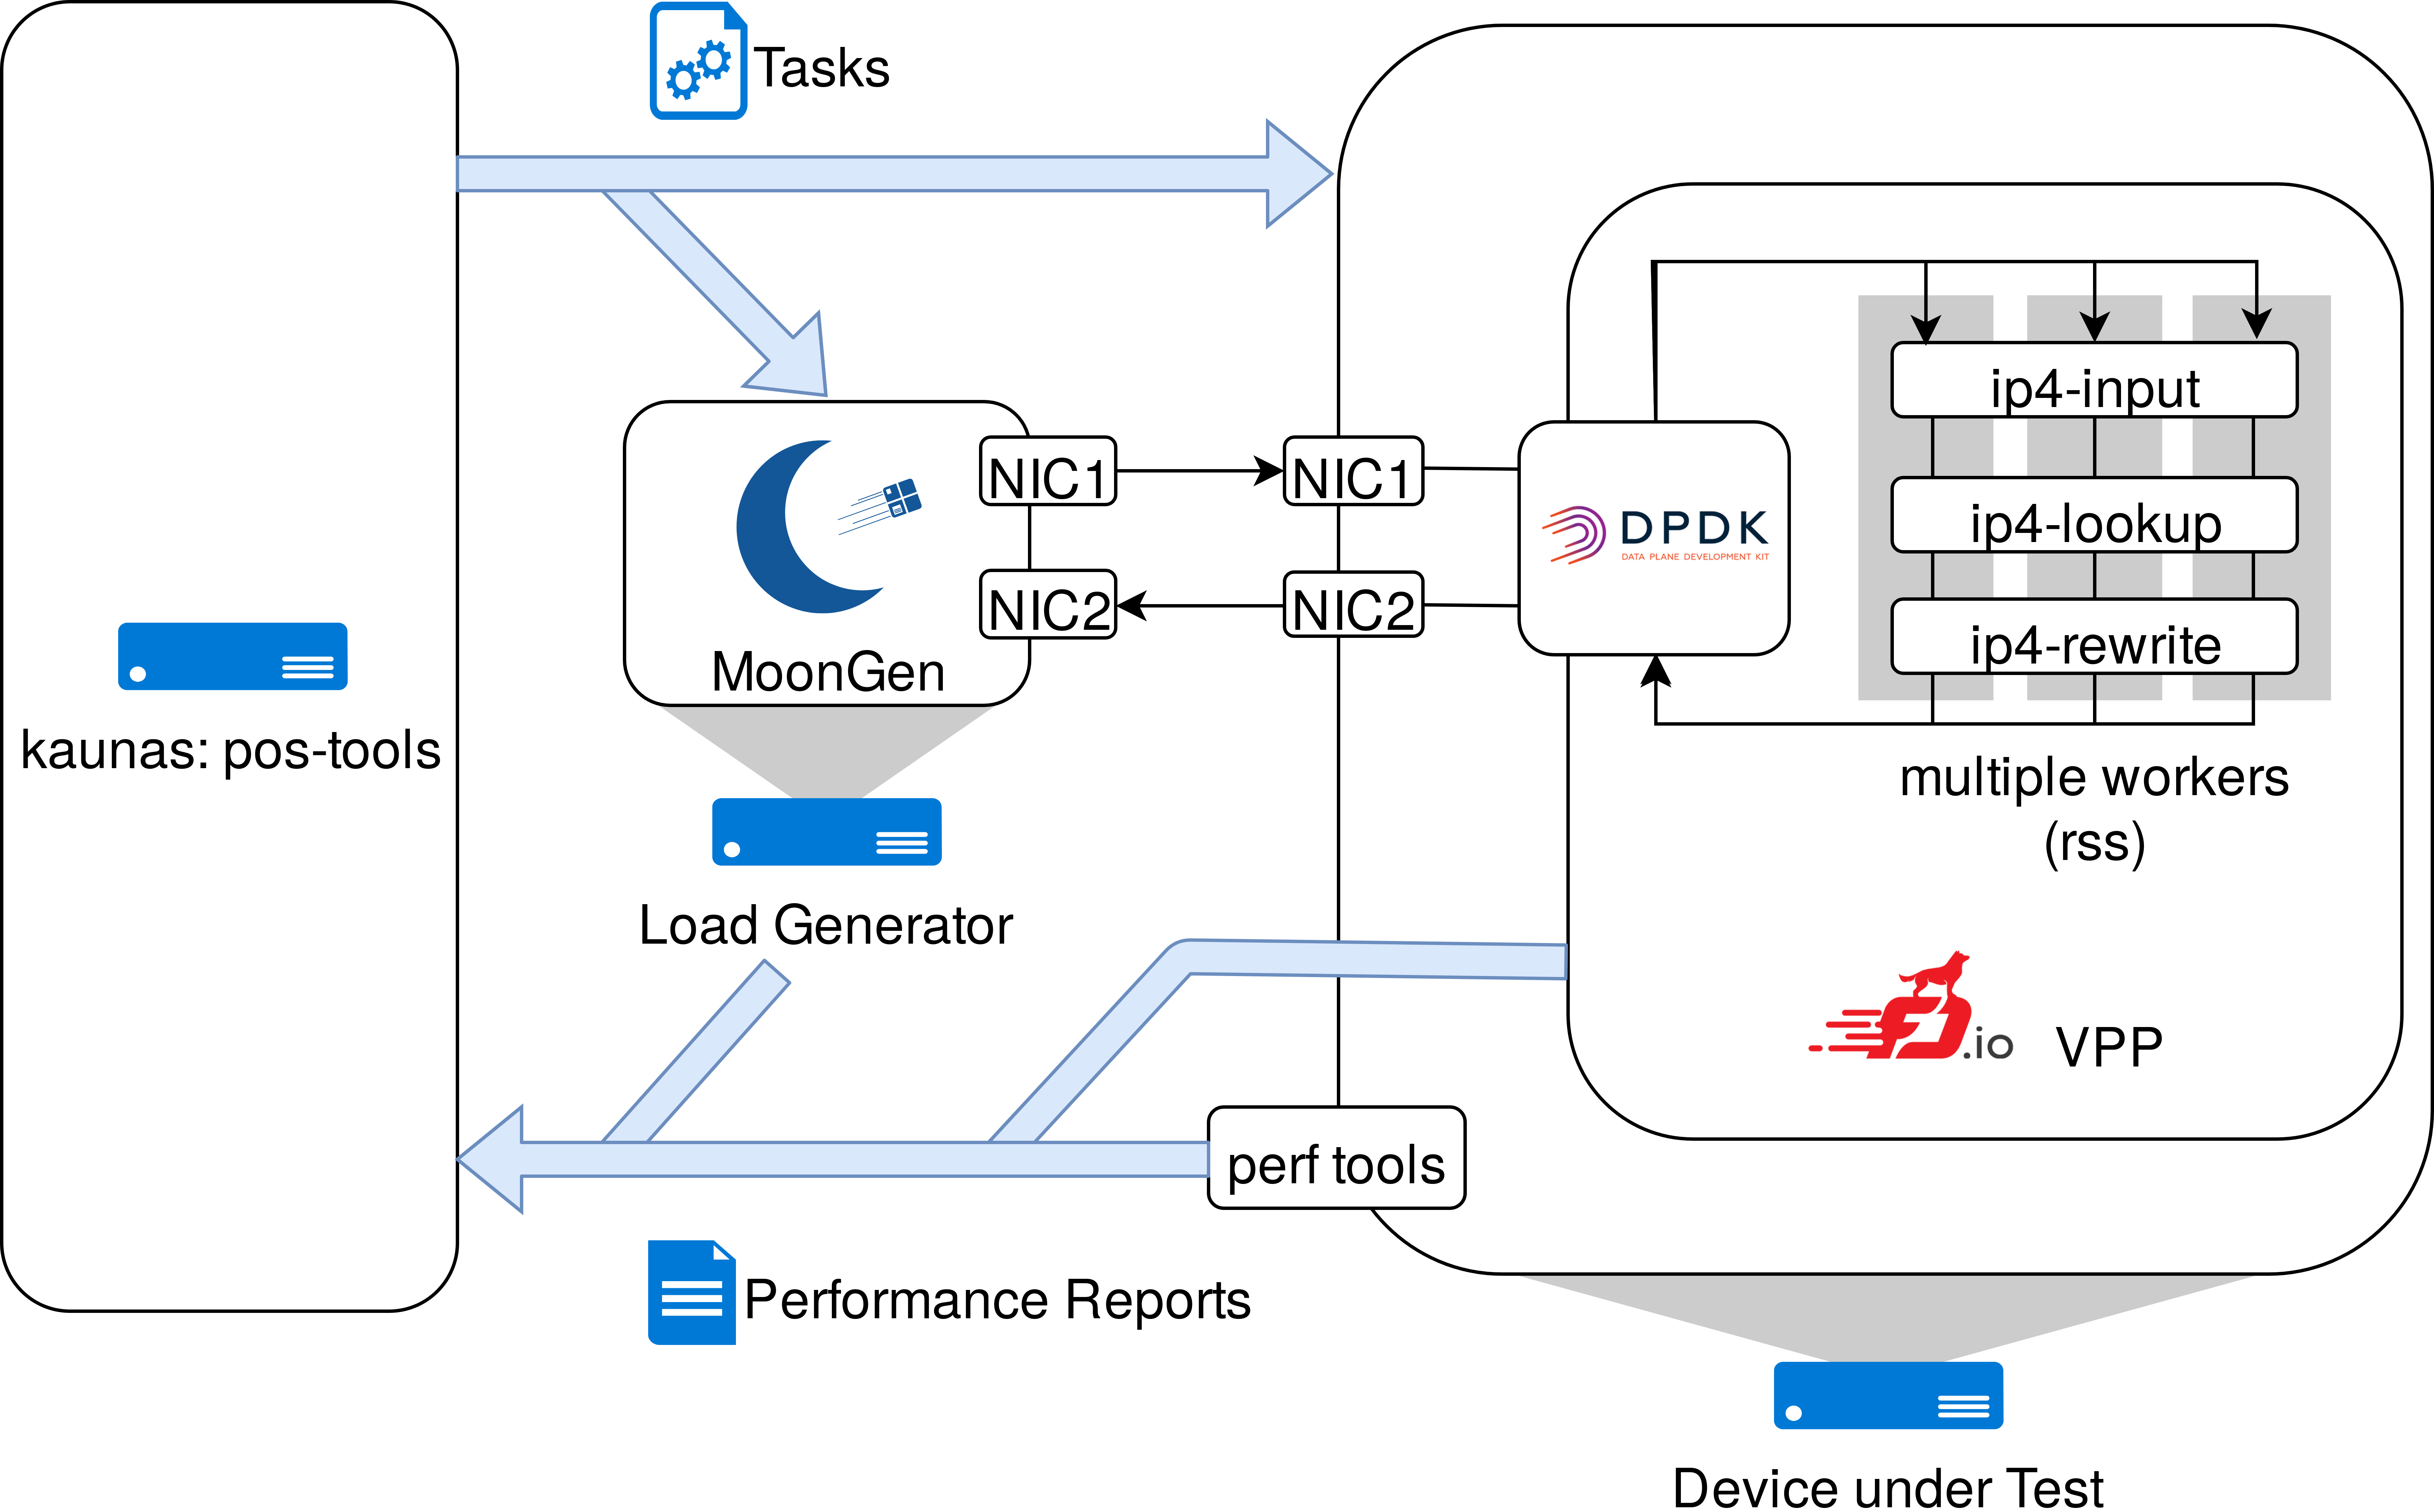
\includegraphics[width=\linewidth]{pics/topology.png}
\caption{Experiment setup for testing VPP with "kaunas" management server, loadgen and DUT}
\label{setup}
\end{figure}


\subsection{Bottlenecks}

\paragraph{Physical Link Speed}
\label{sec:linkspeed}

% - in many cases: 
% 	- 10GbE

Running VPP in with only one worker, the pysical link speed was never
the limiting factor. Usually this is 10GbE in this paper. Only with
multiple worker scenarios the 10Gb/s mark is quickly reached. A simple
way to address this is by testing with bidirectional traffic - sending
load to both of DUT's NIC's and expecting VPP to forward it to both
NIC's again. This way, the load on a single CPU core to be tested can
be doubled, without actually requiring faster links. Other options are
to reduce CPU clock speed or increase the cpu load artificially on a
per-packet basis, in order to create another, even more limiting
bottleneck on the CPU.


\paragraph{Loadgen Speed}

% - loadgen speed
% 	- can saturate a 10GbE link with minimum sized ethernet frames for all tests conducted (14.88mpps)

Another limiting factor could be the load generator's speed of
generating load. MoonGen, the loadgen used for this paper, can
saturate a 10GbE link with minimum sized ethernet frames for all tests
conducted. For a simple unidirectional 10GbE link this results in
14.88mpps \cite{emmerich2015assessing}.

% TODO: remove this if not relevant to the paper: 

Using faster 40GbE with Intel XL710 NICs showed a soft throughput
limit of about 22.81mpps (min. frame size, unidirectional, standard
deviation: 0.22). This was observed with an Intel E5-2620 v3
(2.40GHz). This limit varies when increasing the frame size. Because
reducing the CPU clock speed by 10\% or 50\% results in 12\% and
52\% smaller packet rate, it can be assumed, that this bottleneck lies
within the load generator.

\paragraph{Internal Bandwidth}

% pci bandwidth

Inside the DUT there is first of all the PCI bandwidth. All tested
NIC's are connected by a PCIe 2.0 x8 link with a max transfer rate of
32Gbit/s per direction. In theory a 40GbE link could exceed this
transfer rate. Because the tests in this paper are only done with
small packet sizes, the maximum reached packet generation rate of
around 22.8mpps results in significantly less than 32Gbit/s. For
bigger frame sizes, the PCI bandwidth will become a limiting factor
for 40GbE links.

% ram bandwidth

Sencondly the ethernet frames have to be moved to the main memory. The
test systems use DDR3 memory. It typically supports between 1333 MT/s
(the 10GbE system) or 2133 MT/s (40GbE system) transmitting 64bit per
message. This results in a transfer rate of 85 GBit/s and 136 GBit/s.
This should be sufficient for 10GbE networking, 40GbE links
require at least DDR3-2133 memory. 

\paragraph{CPU time per Packet}

One of the biggest bottlenecks is the CPU time spent per packet, as a
single core can't saturate a 10GbE link. The following subsections
describe how this issue is dealt with in VPP.


% TODO:
% - vpp's cpu cycles: branch prediction, cycles/packet
% - memory latency: latency increases cpu time, caches can improve latency


\subsection{NICs with DPDK and VPP}

For VPP to utilize NIC's up to their specified line rate, it relies on
\Ac{dpdk}. This introduces a few noteworthy optimizations:

\paragraph{RSS (Receive Side Scaling)}

When the NIC recieves a packet, it can be configured to hash over
specified packet header fields to assign the packet to a recieving
queue. The idea is, to efficiently separate for example different ip
traffic flows early which can then be processed by several VPP workers
concurrently and independently. \cite{linguaglossa2017high}

\paragraph{Zero-Copy}

Because memory bandwidth is actually limited, it is important not to
move frames around unnecessarily. Therefore the NIC copys the recieved
frames to memory shared with VPP which is their final fixed
location. \cite{linguaglossa2017high}

\paragraph{Busy Polling}

Newer VPP versions have options to be notified about new packets in
the shared memory via interrupts - or, better suited for high
performance applications, vpp workers can be busy polling.

% TODO
% vpp's multithreading model: hqos, worker, main thread
% placement

\subsection{Packet Processing Graph}

% - modularity, feature rich
%	- visualize the parsing done in the first step as in the vpp paper and explain 
% 		bridging only: ip header parsing slowdown behaviour

VPP's packet processing is defined by the packet processing graph.
Figure \ref{nodegraph} illustrates selected packet paths important for
this paper. Depending on the plugins and configuration in place, this
graph can be customized for example to replace specific software
functions with hardware accelerators. Depending on the initial packet
parsing which happens in the "dpdk-input" and "l2-input" nodes, the
packets traverse the graph over their respective paths.

\paragraph{xconnect}

Static layer 2 connections between physical links (xconnect) are
parsed and passed through the dpdk-, ethernet- and l2-input nodes and
only use the l2-output node to be sent to the target device.

\paragraph{Bridging}

With bridged configurations, packets are treated the same as xconnect
traffic, but there is an additional l2-fwd node which looks up the
destination in the layer 2 \Ac{fib}. Packets for this node are
processed by \lstinline|l2fwd_node_inline| implemented
\lstinline|vpp/src/vnet/l2/l2_fwd.c|.

\paragraph{IPv4}
\label{sec:headerparsing} 

The ip4 path shares it's packet header parsing with the layer 2
processing graph. After it's parsing of a \Ac{udp} packet, the
ip4-lookup and ip4-rewrite nodes implemented by the
\lstinline|ip4_lookup_inline| and the \lstinline|ip4_rewrite_inline|
function in \lstinline|vpp/src/vnet/ip/ip4_forward.c| take care of
looking up the next-hop destination and rewriting the packet header.
Their predecessing node (ip4-input) is also predecessor for other ip4
protocol nodes like for example ICMPv4. A lot of the header parsing
happens before the ip4-input node though, even if this information may
not be needed for the followup nodes.

\paragraph{IPv6}

The ip6 packet processing path differs completely from the previously
discussed paths, because it implements it's own parsing in the
ip6-input node. For lookup and forwarding purpose, there follow an
ip6-lookup and an ip6-rewrite node, similar like the ip4 path. Those
nodes are implemented by the \lstinline|ip6_lookup| and the
\lstinline|ip6_rewrite| function in
\lstinline|vpp/src/vnet/ip/ip6_forward.c|.

\begin{figure}[!ht]
\noindent\hspace{0.5mm}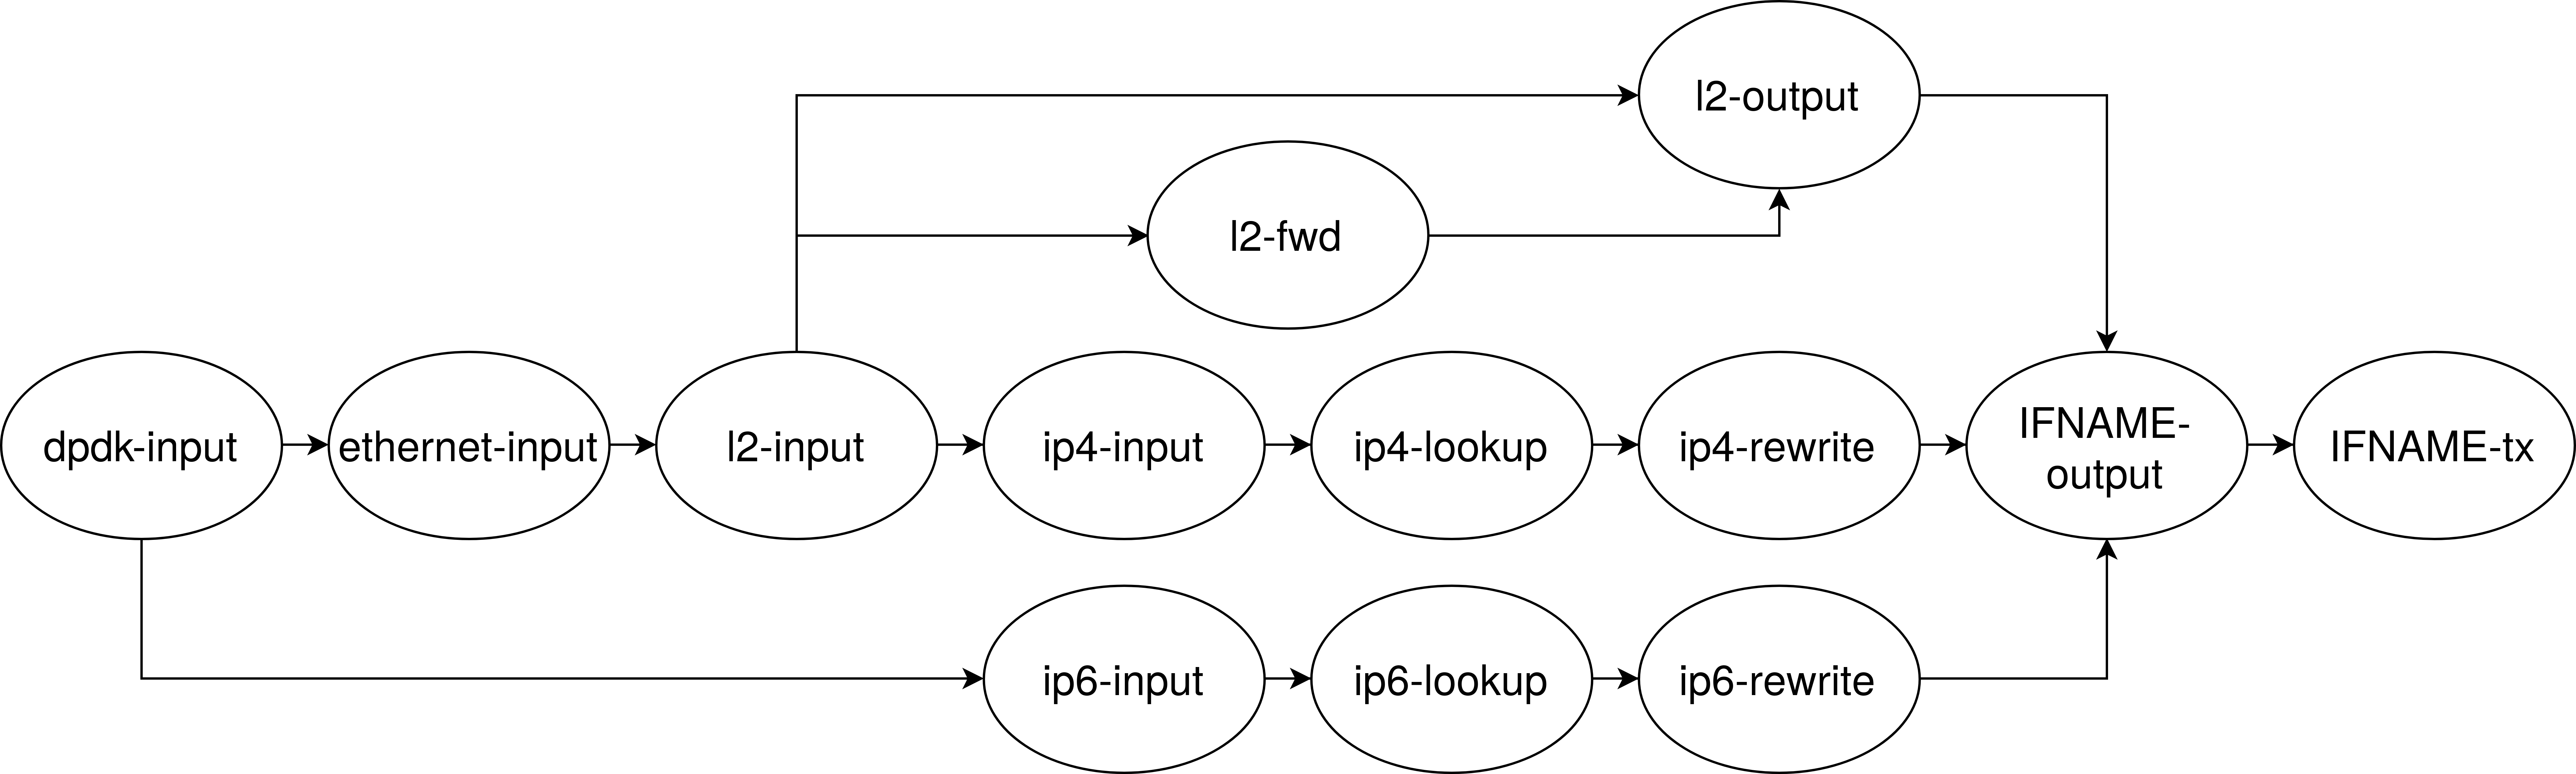
\includegraphics[width=\linewidth]{pics/vpp-nodes-horizontal.png}
\caption{VPP packet processing graph for xconnect, bridging, ip4 routing and ip6 routing. Other paths are left out. }
\label{nodegraph}
\end{figure}

 
\subsection{VPP's forwarding datastructures}

VPP implements several datastructures for their packet forwarding. A
BiHash table is used for the layer 2 \Ac{fib} and the ip6 \Ac{fib}
(\lstinline|vpp/src/vppinfra/bihash*|) \cite{vppwiki:bihash}. IPv4 \Ac{fib}
lookups use a mtrie (\lstinline|vpp/src/vnet/ip/ip4_mtrie.h|).

% There is a  All of them are used to heavily utilize the CPU's cache.

\paragraph{l2-fib}

For packets reaching the l2-fwd node, the destination lookup is done
for example by \lstinline|l2fib_lookup_4| in
\lstinline|vpp/src/vnet/l2/l2_fib.h|. 

Each lookup takes a 64 bit \lstinline|l2fib_entry_key_t| containing
the mac address and the bridge domain index of the incoming interface.
It returns a 64 bit \lstinline|l2fib_entry_result_t| with the relevant
destination information. 

% one entry cache in l2fib_lookup

\paragraph{ip4-fib}

% hashset vpp/vppinfra/hash.*

% show ip fib and ip4fib functions vpp/src/vnet/fib/ip4_fib.c
% contains ip4_fib_t def.

% ip4-lookup node vpp/src/vnet/ip/ip4_forward.c
% used mtrie: vpp/src/vnet/ip/ip4_mtrie.*

% ip_adjencency_t contains all information about the next hop
% vpp/src/vnet/adj/adj.h

The ip4 lookup is implemented by \lstinline|ip4_fib_table_lookup| in
\lstinline|vpp/src/vnet/fib/ip4_fib.h|. The \Ac{fib} struct
\lstinline|ip4_fib_t| contains two data structures. A list of hash
tables (implemented in \lstinline|vpp/vppinfra/hash.h|), one for each
ip prefix length, which is only used for \Ac{cli} status creation and
to enforce unique inserts. The second data structure is used by the
ip4-lookup node for ip4 \Ac{fib} lookups. The mtrie lookup results in
an adjecency index which is then used by the ip4-rewrite node to
rewrite the destination. Therefore the rewrite node gets the
\lstinline|ip_adjacency_t|\footnote{\lstinline|ip_adjecency_t| is
defined in \lstinline|vpp/src/vnet/adj/adj.h|} information from the
respective adjecency vector according to the adjecency index.

% ip4_lookup_inline prefetch header and frame for next packet badge

\paragraph{ip6-fib}

The ip6 \Ac{fib} lookup itself is done by the ip6-lookup node and
implemented by \lstinline|ip6_fib_table_fwding_lookup| in
\lstinline|vpp/src/vnet/fib/ip6_fib.h| and uses the BiHash table for
lookups in the ip6-lookup node. The lookup returns an 32 bit adjecency
index which will be used by the ip6-rewrite node to get the next
packet destination from the \lstinline|ip_adjencency_t| vector, just
like the ip4-rewrite node does.

% ip4_lookup_inline prefetch header and frame for next packet badge

% table size problems

\subsection{Vectorization}

% - vectorization
% 	- low level optimization for caches
%	- more efficient instruction cache usage?
%	- VLIB_FRAME_SIZE


\subsection{Collected Data}

% why used testing methods: latency, throughput, perf/cache-misses

% Analyzes and assesses several possible approaches that solve the problem



